%---------------------------------------------------------------------------------------- % THE CHICAGO STYLE  %----------------------------------------------------------------------------------------

\chapter{Chicago style}

\section{Formatting the Chicago essay}

When setting up your word processor for a Chicago-formatted document, use the
following settings and rules:

\begin{itemize} 

\item Use one-inch margins on all sides of the document. 

\item Place the page number on the right side of each page in the
document's header. If instructed to do so by a professor, include your last name before the page number on each page. 

\item Double space the document. 

\item Block quotes are formed when a quote runs more than 100 words. Indent the entire  block of text
with a 1/2-inch tab from the left margin. 
\item Endnotes and bibliographic entries are single-spaced with a blank line separating them. 
\item Indent the first line of a note entry with a 1/2-inch tab. 
\item Indent the second, and any subsequent, line of a bibliographic entry with a 1/2-inch tab. 
\item The Chicago form requires a title page. The title of the essay is centered about  1/3 down
the top of the page. Place your name, course information, and date on three
separate, centered lines at the center of the document.
\end{itemize}
\bigskip

\begin{center}
\begin{tcolorbox}[colframe=oyster, coltitle=black, sharp corners, title=\ding{52} Note!]
The title page is \emph{counted but not
numbered}. Therefore,  begin your essay with page 2.
\end{tcolorbox}
\end{center}

\section{A model of the Chicago essay} \newpage 

%\begin{center}
%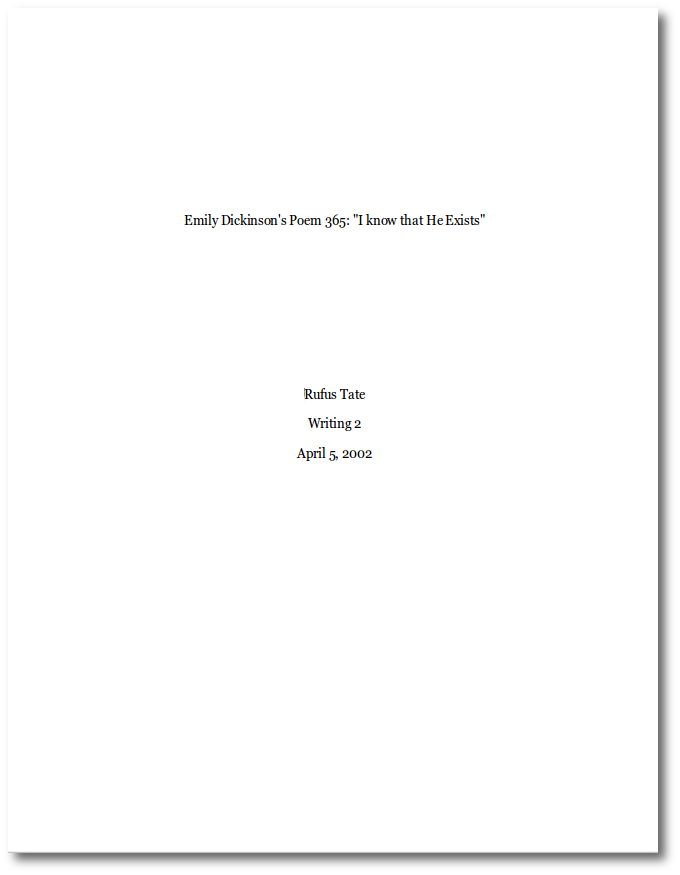
\includegraphics[width=.50\textwidth]{chicagotitle} \end{center}

\begin{tcolorbox}[enhanced,width=4.2in,left=.3in, right=.3in,
   drop fuzzy shadow southeast,
    boxrule=0.4pt,sharp corners,colframe=black!80!black,colback=white!10]

{\scriptsize 

\vspace{3.5cm}

\begin{center}Emily Dickenson's Poem \#365: "I know that He exists"
\vspace{3cm}

Rufus Tate

\vspace{5cm}
Writing 002

Dr. Clem Spanning

October 28, \the\year \end{center}

}

\vspace{.55cm}
\end{tcolorbox}

\newpage

%\begin{center} 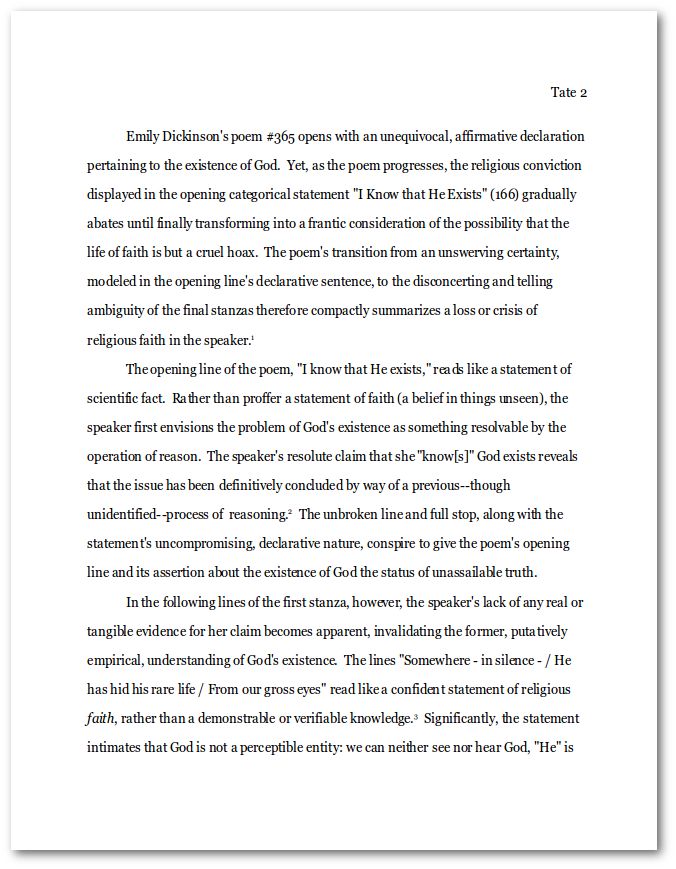
\includegraphics[width=.50\textwidth]{chicago2} \end{center}

\bigskip

\begin{tcolorbox}[enhanced,width=4.2in,left=.3in, right=.3in,
   drop fuzzy shadow southeast,
    boxrule=0.4pt,sharp corners,colframe=black!80!black,colback=white!10]

\medskip

{\scriptsize \begin{flushright} Tate 2 \end{flushright}
\begin{doublespacing}


\hspace{1.4em} Emily Dickinson's poem \#365 opens with an unequivocal, affirmative declaration pertaining to the existence of God.  Yet, as the poem progresses, the religious conviction displayed in the opening categorical statement "I Know that He Exists" gradually abates until finally transforming into a frantic consideration of the possibility that the life of faith is but a cruel hoax.  The poem's transition from an unswerving certainty, modeled in the opening line's declarative sentence, to the disconcerting and telling ambiguity of the final stanzas therefore compactly summarizes a loss or crisis of religious faith in the speaker.\textsuperscript{1}  
  
\hspace{1.4em} The opening line of the poem, "I know that He exists," reads like a statement of scientific fact.  Rather than proffer a statement of faith (a belief in things unseen), the speaker first envisions the problem of God's existence as something resolvable by the operation of reason.  The speaker's resolute claim that she "know[s]" God exists reveals that the issue has been definitively concluded by way of a previous--though unidentified--process of  reasoning.  The unbroken line and full stop, along with the statement's uncompromising, declarative nature, conspire to give the poem's opening line and its assertion about the existence of God the status of unassailable truth.  

\hspace{1.4em}In the following lines of the first stanza, however, the speaker's lack of any real or tangible evidence for her claim becomes apparent, invalidating the former, putatively empirical, understanding of God's existence. The lines "Somewhere - in silence - / He has hid his rare life / From our gross eyes" read like a confident statement of religious faith, rather than a demonstrable or verifiable knowledge.\textsuperscript{2}  Significantly, the statement intimates that God is not a perceptible entity: we can neither see nor hear God, "He" is both hidden "Somewhere - in Silence" and away "From our gross eyes." 


\end{doublespacing}}
\vspace{.33in}


\end{tcolorbox}

\section {In-text citations}

In the Chicago form, an in-text citation is indicated by a superscript number
resembling the following:

\begin{quote} Recent scholarship on the concept of sovereignty has displayed a
remarkable lack of interest in the role of private property.\textsuperscript{7}
\end{quote}

\noindent This in-text reference will correspond to a citation on the Notes page
at the conclusion of the document, such as this one:

\begin{singlespace}
\begin{quote} \hspace{.4in}7. Giorgio Agamben, \emph{Homo Sacer: Sovereign Power
and Bare Life} (Stanford: Stanford University Press, 1998), 96. \end{quote}
\end{singlespace}

\section{The Notes page}

In the Chicago style, the endnotes appear on what is known as the \textbf{Notes}
page\textemdash a separate page that directly follows the conclusion of the
essay. The Notes page is organized as a numbered list that presents each
citation in the order that it appears within the essay. Thus, your first
citation will be note 1, your second will be note 2, and so on.

\section{Setting up the Notes page} When setting up the Notes page, use the
following rules:

\begin{itemize} \item Center the word "Notes" at the top of the page. \item
Single-space the endnotes with a line separating entries. \item Indent the first
line of an endnote entry with a 1/2-inch tab. \end{itemize}

\newpage
\section{Example Chicago Notes page} 

\begin{tcolorbox}[enhanced,width=4.2in,left=.3in, right=.3in,
   drop fuzzy shadow southeast,
    boxrule=0.4pt,sharp corners,colframe=black!80!black,colback=white!10]

\medskip

{\scriptsize \begin{flushright} Tate 12 \end{flushright}
\begin{singlespacing}

\begin{center} Notes \end{center}

\hspace{2em}1. Lance Carter, \emph{On Building Copper Stills} (New York: Random House, 1988), 10.\\

\hspace{2em}2. Ibid., 20.\\

\hspace{2em}3. George Crary, \emph{The Silence of Pigs} (1879; reprint, New York: Faber Books, 2010), 100.\\

\hspace{2em}4. Ibid.\\

\hspace{2em}5. Ibid.\\

\hspace{2em}6. Ibid., 2.\\

\hspace{2em}7. Ibid., 22.\\

\hspace{2em}8. Ibid., 7.\\ 

\hspace{2em}9. Jonas Whale, "The Southern Mystique," in \emph{Faulkner's Mississippi Drinkers}, ed. Gray Davis (Chattanooga: University of Tennessee Press, 2000), 99.\\

\hspace{2em}10. Ibid., 8.\\

\hspace{2em}11. Crary, \emph{Silence}, 45.\\

\hspace{2em}12. Jedediah Cross, \emph{Woods, Bear, and Corn} (Danville: White Lightning Books, 1988), 12.\\

\hspace{2em}13. Crary, \emph{Silence}, 45.\\

\hspace{2em}14. Ibid.\\

\hspace{2em}15. Rufus Tate, \emph{Lipstick on a Pig} (New York: Goose Pimple Press, 1988), 70.\\

\hspace{2em}16. Ibid., 31.\\

\hspace{2em}17. William T. Bibble, "Farming Your Way to Millions," \emph{Alabama Agriculture} 4, no. 8 (1979): 20.\\


\end{singlespacing}
}
\bigskip


\end{tcolorbox}

\newpage

\section{Rules for making the notes} The Chicago form uses an economical
practice that reduces the  work involved in presenting the essay's footnotes or
endnotes. While this design  ultimately means less typing, a number of strict
rules must be followed:

\begin{itemize} \item Present the citations in the numerical order as they
appear within the text.

\item The first time a source is cited, use the \emph{full} Chicago notes form.

\item If the same source is used more than once, the \emph{shorthand} version of
the Chicago  notes form is used the second (and each subsequent) time. The
shorthand version  contains \textbf{a)} the author's last name, \textbf{b)} a
shortened version of the title,  and \textbf{c)} the page number(s) of the
citation.

\item If a single source is used twice or more in a row, the Latin abbreviation
"Ibid." is  used along with the page number, rather than the shorthand version
of the form.  (Ibid. means "in the same place.")

\item If the same source is used \emph{twice in a row} and the citation \emph{is
from  the same page as the previous citation}, "Ibid." is used by itself without
the  page number.  \end{itemize}

\section{The Bibliography page} The Chicago style also requires that you include
a bibliography page at the conclusion of your essay. As you will see in the next
section, the bibliography  form differs slightly from the notes form, so take
care to use the correct one. To format the bibliography page, use the following
rules:

\begin{itemize} \item Place the bibliography page after the notes page. \item
Center the word "Bibliography" at the top of the page. \item Single-space
entries with a line separating entries. \item Alphabetize by the author's last
name. \item Indent the second (and any subsequent) line of an entry with a
1/2-inch tab. \end{itemize}

\newpage \section{Example Chicago Bibliography page} 
\begin{tcolorbox}[enhanced,width=4.2in,left=.3in, right=.3in,
   drop fuzzy shadow southeast,
    boxrule=0.4pt,sharp corners,colframe=black!80!black,colback=white!10]

\medskip

{\scriptsize \begin{flushright} Tate 12 \end{flushright}
\begin{singlespacing}

\begin{center}Bibliography \end{center}

\hangindent2em{Allen, Tate. \emph{White Lightning}. Edited by Leon Edel. Boston: Houghton, 1963.}\\

\hangindent2em{Fulton, Fendal. \emph{Bootleggers and the Birth of NASCAR}. Legrange: Automotive Books, 1974.}\\

\hangindent3em{Graves, Thomas. "Building a Copper Worm." In \emph{An American Art: Illegal Moonshine and the Foxfire Tradition}, edited by Eric Foner, 77-88. Atlanta: McKinley and Smith, 2011.}\\

\hangindent3em{Knox, John. Introduction to \emph{The Life of Popcorn Sutton}, by Elders Johnson, 2-9. New York: Random House, 2009.}\\

\hangindent3em{Linter, Jerry S. Review of \emph{The Orchard Revival}, by Cormac Freedman. \emph{Tennessee
Literary Review} 120, no. 4 (1998): 20-23.}\\

\hangindent3em{Mellon, Batson. \emph{A History of the Tennessee Valley: 1780-1980}. Baltimore: Brown Bag Press, 1998.}\\

\hangindent3em{Robers, John, Philip Glass and Jane Hinds. \emph{Mason Jars and Corn Whiskey}. Boston: University of Tennessee Press, 2000.}\\

\hangindent3em{Talmage, Lance. \emph{Copper Stills in Appalachia}. New York: Random House, 1988.}\\

\hangindent3em{Zeb, Fred and Linda Tanner, eds. \emph{Anarchy on the River's Edge}. Chattanooga: Lookout Publishing, 1974.}\\

\hangindent3em{Zoltan, Hayden. "Southern Tradition as Politics." \emph{American Folkways} 45, no. 6 (2010): 45-61. doi: 12.2398/ahl.483.1.112.}\\


\end{singlespacing}}
\vspace{3.2cm}

\end{tcolorbox}

\newpage

\section{The Chicago Bibliography}

The following section provides examples for citing sources that are commonly
found in academic writing. The various forms have been organized into sections 
on \textbf{books}, \textbf{periodicals}, \textbf{electronic sources}, and
\textbf{other types of sources} that are less common.

\begin{itemize}
\item In each form, the first citation is the \textbf{bibliography} form and the
second citation is the \textbf{notes} form.
\end{itemize}

\section{Book forms}

\subsection{A book by one author}


\begin{center}{Bibliography}\end{center}

\begin{singlespace}
\noindent\hangindent1.2cm {Taylor, Herman. \emph{A Tale of One City}. New York:
Little and Sons, 1998.}
\end{singlespace}




\begin{center}{Notes}\end{center} 
\begin{singlespace}
\noindent\hspace{1.2cm}1. Herman Taylor,
\emph{A Tale of One City} (New York: Little and Sons, 1998), 77.
\end{singlespace}


\subsection{Multiple authors}


\begin{center}{Bibliography}\end{center}

\begin{singlespace}
\noindent\hangindent1.2cm{Roberts, John, Philip Glass and Jane Hinds.
\emph{Recovering the City of Boston}. Boston: University of Massachusetts Press,
2000.}
\end{singlespace}


\begin{center}{Notes}\end{center}
\begin{singlespace}
\noindent\hspace{1.2cm}1. John Roberts, Philip Glass and Jane Hinds,
\emph{Recovering the City} \emph{of Boston} (Boston: University of Massachusetts
Press, 2000), 77.
\end{singlespace}



\begin{itemize} \item Include up to three authors in the \textbf{notes} form.
\item If there are four or more, give the first author's name and then use "et.
al." ("and others") to replace the other authors.  \item In the
\textbf{bibliography} form, include up to ten authors. If there are more than
ten authors, give the first seven and then use "et. al." \end{itemize}

\subsection{A book with an editor}

    
\begin{center}{Bibliography}\end{center}
\begin{singlespace}
\noindent\hangindent1.2cm{James, Henry. \emph{Portrait of a Lady}. Edited by
Leon Edel. Boston: Houghton, 1963.}
\end{singlespace}

\begin{center}{Notes}\end{center}
\begin{singlespace}
\noindent\hspace{1.2cm}12. Henry James, \emph{Portrait of a Lady}, ed. Leon Edel
(Boston: Houghton, 1963), 77.
\end{singlespace}


\subsection{Book with editor only}

\begin{center}{Bibliography}\end{center}
\begin{singlespace}
\noindent\hangindent1.2cm{Smith, Edward, ed. \emph{Stuck in Goshen}. Nashville:
Greenwood Press, 1963.}\\

\noindent\hangindent1.2cm{Zebe, Fred and Linda Tanner, eds. \emph{Anarchy on the
River's Edge}. Chattanooga: Lookout Publishing, 1974.}
\end{singlespace}

\begin{center}{Notes}\end{center}
\begin{singlespace}
\hspace{1.2cm}17. Edward Smith, ed., \emph{Stuck in Goshen} (Nashville:
Greenwood Press, 1963), 77.\\

\noindent\hspace{1.2cm}18. Fred Zebe and Linda Tanner, eds., \emph{Anarchy on the River's
Edge}. (Chattanooga: Lookout Publishing, 1974), 77.
\end{singlespace}

\begin{itemize} \item If there are multiple editors, use "eds." \end{itemize}

\subsection{An edition (other than the first)}
\begin{center}{Bibliography}\end{center}

\begin{singlespace}
\noindent\hangindent1.2cm{Thompson, Fred. \emph{Why I Fight}. 3rd ed. New York:
Vanity Publications, 2000.}
\end{singlespace}

\begin{center}{Notes}\end{center}

\begin{singlespace}
\noindent\hspace{1.2cm}12. Fred Thompson, \emph{Why I Fight}, 3rd. ed. (New
York: Vanity Publications, 2000), 77.
\end{singlespace}

\subsection{Corporate author (written by organization or government)}

\begin{singlespace}
\begin{center}{Bibliography}\end{center} \noindent\hangindent1.2cm{John Bigan
Society. \emph{The Religions of Kenya}. New York: John Bigan Publishing, 2000.}
\end{singlespace}

\begin{center}{Notes}\end{center} 
\begin{singlespace}
\noindent\hspace{1.2cm}10. John Bigan Society,
\emph{The Religions of Kenya} (New York: John Bigan Publishing, 2000), 77.
\end{singlespace}

\subsection{An anthology} \begin{center}{Bibliography}\end{center}

\begin{singlespace}
\noindent\hangindent1.2cm{Foner, Eric, ed. \emph{An American Voice: A Collection
of America's Finest Essays}. Boston: McKinley and Smith, 2011.}
\end{singlespace}

\begin{center}{Notes}\end{center} 

\begin{singlespace}
\noindent\hspace{1.2cm}15. Eric Foner, ed.,
\emph{An American Voice: A Collection of America's Finest Essays} (Boston:
McKinley and Smith, 2011), 77.
\end{singlespace}


\subsection{Work in an anthology}

\begin{singlespace}
\begin{center}{Bibliography}\end{center} \noindent\hangindent1.2cm{Graves,
Thomas. "The History of our National Anthem." In \emph{An American Voice: A
Collection of America's Finest Essays}, edited by Eric Foner, 77-88. Boston:
McKinley and Smith, 2011.}
\end{singlespace}


\begin{center}{Notes}\end{center} 

\begin{singlespace}
\noindent\hspace{1.2cm}13. Thomas Graves, "The
History of our National Anthem," in \emph{An American Voice: A Collection of
America's Finest Essays}, ed. Eric Foner (Boston: McKinley and Smith, 2011),
77-88.
\end{singlespace}
\subsection{No author or editor}

\begin{center}{Bibliography}\end{center}

\begin{singlespace}
\noindent\hangindent1.2cm{\emph{A Wicked Guide to Boston}. Boston: Beantown
Publishing, 2000.}
\end{singlespace}


\begin{center}{Notes}\end{center} 
\begin{singlespace}
\noindent\hspace{1.2cm}25. \emph{A Wicked Guide to Boston} (Boston: Beantown Publishing, 2000), 22.
\end{singlespace}


\subsection{Introduction, preface, forward or afterward}
\begin{center}{Bibliography}\end{center} 

\begin{singlespace}
\noindent\hangindent1.2cm{Knox, John.
Introduction to \emph{The Life of James}, by Elders Johnson, 2-9. New York:
Random House, 2009.}
\end{singlespace}


\begin{center}{Notes}\end{center} 
\begin{singlespace}
\noindent\hspace{1.2cm}33. John Knox,
introduction to \emph{The Life of James}, by Elders Johnson (New York: Random
House, 2009), 7.
\end{singlespace}


\begin{itemize}\item Substitute the word introduction with preface, afterward,
or foreward as needed.\end{itemize}

\subsection{Book with a translator}

\begin{center}{Bibliography}\end{center} 

\begin{singlespace}
\noindent\hangindent1.2cm{McDougle,
Astrid. \emph{The Basics of Gaelic}. Translated by Paddy Maloney. New York:
Vintage, 1990.}
\end{singlespace}

\begin{center}{Notes}\end{center} 

\begin{singlespace}
\noindent\hspace{1.2cm}45. Astrid McDougle,
\emph{The Basics of Gaelic}, trans. Paddy Maloney (New York: Vintage, 1990), 22.
\end{singlespace}


\subsection{Multivolume work}

\begin{center}{Bibliography}\end{center} 

\begin{singlespace}
\noindent\hangindent1.2cm{Graves,
Johanna. \emph{Ronald Reagan and the Iran-Contra Affair}. Vol. 7. New York:
Greenstalk, 1988.}
\end{singlespace}


\begin{center}{Notes}\end{center} 
\begin{singlespace}
\noindent\hspace{1.2cm}23. Johanna Graves,
\emph{Ronald Reagan and the Iran-Contra Affair}, vol. 7 (New York: Greenstalk,
1988), 77.
\end{singlespace}


\begin{itemize}\item If the volume has a separate title, place a comma after the
volume number and enter its name in italics.\end{itemize}

\subsection{Book in a series}

\begin{center}{Bibliography}\end{center} 

\begin{singlespace}
\noindent\hangindent1.2cm{Smith, Rod.
\emph{American Economic Expansion in the Gilded Age}. American Economic History
Series. New York: Grim and Drang, 1988.}
\end{singlespace}


\begin{center}{Notes}\end{center} 

\begin{singlespace}
\noindent\hspace{1.2cm}44. Rod Smith,
\emph{American Economic Expansion in the Gilded Age}, American Economic History
Series (New York: Grim and Drang, 1988), 78.
\end{singlespace}

\subsection{Republished Book}

\begin{singlespace}
\begin{center}{Bibliography}\end{center} \noindent\hangindent1.2cm{Cranston,
Brian. \emph{Outlooks on Faith and Reason}. 1979. Reprint, New York: Stroke and
Crowder, 2000.}
\end{singlespace}

\begin{center}{Notes}\end{center} 

\begin{singlespace}
\noindent\hspace{1.2cm}44. Brian Cranston,
\emph{Outlooks on Faith and Reason} (1979; reprint, New York: Stroke and
Crowder, 2000), 9.
\end{singlespace}


\subsection{Article in a reference work, such as a dictionary or encyclopedia}

\begin{center}{Notes}\end{center} 

\begin{singlespace}
\noindent\hspace{1.2cm}7.
\emph{Merriam-Webster's Collegiate Dictionary}, 10th ed., s.v. "Suzerian."
\end{singlespace}


\begin{itemize}\item Well-known reference sources, such as encyclopedias or
dictionaries, that are arranged alphabetically by word or term do not require
page numbers or need to be included in your bibliography. Abbreviate the Latin
term \emph{sub verbo}, or "under the word," in your note to indicate
this.\end{itemize}

\subsection{Sacred texts} \begin{center}{Notes}\end{center}
\begin{singlespace}
\noindent\hspace{1.2cm}22. Genesis 2: 2-5 (New International Version).
\end{singlespace}

\begin{itemize}\item For sacred texts such as the Bible, Koran, or Torah, cite
the work in your notes, but not the bibliography. In the note, provide
information about the chapter and verse, but not the page number. If there is a
version, put that information in parenthesis after the chapter and verse
information. \end{itemize}

\subsection{Book with title within the title}

\begin{center}{Bibliography}\end{center} 

\begin{singlespace}
\noindent\hangindent1.2cm{Hixson, Fred.
\emph{On Cormac McCarthy's} Blood Meridian. New York: Plainspeak Press, 2000.}
\end{singlespace}

\begin{center}{Notes}\end{center} 

\begin{singlespace}\noindent\hspace{1.2cm}45. Fred Hixon,
\emph{On Cormac McCarthy's} Blood Meridian (New York: Plainspeak Press, 2000),
56.
\end{singlespace}

\begin{itemize}\item If a book title contains the title of another book, remove
the italics to indicate the title of the other work.\end{itemize}

%--------------------------------------------------------------------------------------------
%Periodicals %-------------------------------------------------------------------------------------------

\section{Periodical forms}

\subsection{Article in a scholarly journal}

\begin{center}{Bibliography}\end{center} 

\begin{singlespace}
\noindent\hangindent1.2cm{Taylor,
James. "The Indian Matter of Charles Brockden Brown's \emph{Edgar Huntly}."
\emph{American Literature} 45, no. 6 (1998): 432-45.}
\end{singlespace}


\begin{center}{Notes}\end{center} 

\begin{singlespace}
\noindent\hspace{1.2cm}19. James Taylor, "The
Indian Matter of Charles Brockden Brown's \emph{Edgar Huntly}," \emph{American
Literature} 45, no. 6 (1998): 434.
\end{singlespace}

\subsection{Article in a newspaper}

\begin{center}{Bibliography}\end{center} 

\begin{singlespace}
\noindent\hangindent1.2cm{McKinley,
Robert. "Cat Saved from Dog." \emph{New York Times}, October 28, 2000, early
edition, sec. B.}
\end{singlespace}

\begin{center}{Notes}\end{center} 

\begin{singlespace}
\noindent\hspace{1.2cm}21. Robert McKinley,
"Cat Saved from Dog," \emph{New York Times}, October 28, 2000, early edition,
sec. B.
\end{singlespace}

\begin{itemize}\item If there is no section or edition information, end with the
year of publication.\end{itemize}

\subsection{A review}

\begin{center}{Bibliography}\end{center} 

\begin{singlespace}
\noindent\hangindent1.2cm{Smith, Jerry
S. Review of \emph{The Orchard Revival}, by Cormac Freedman. \emph{Oregon
Literary Review} 120, no. 4 (1998): 20-23.}
\end{singlespace}

\begin{center}{Notes}\end{center} 
\begin{singlespace}
\noindent\hspace{1.2cm}43. Jerry S. Smith,
review of \emph{The Orchard Revival}, by Cormac Freedman, \emph{Oregon Literary
Review} 120, no. 4 (1998): 22.
\end{singlespace}

\subsection{An unsigned article}

\begin{center}{Bibliography}\end{center} 
\begin{singlespace}
\noindent\hangindent1.2cm{"A Walk Down
Nostalgia Lane." \emph{Bloomington Sun} October 20, 2013, sec. B6.}
\end{singlespace}

\begin{center}{Notes}\end{center} 
\begin{singlespace}
\noindent\hspace{1.2cm}21. \emph{Bloomington
Sun}. "A Walk Down Nostalgia Lane." October 20, 2013, sec. B6.
\end{singlespace}

\begin{itemize}\item In an unsigned article, state the article title first in
the note. In the bibliography, begin with the name of the
publication.\end{itemize}

\subsection{Article in a magazine}

\begin{center}{Bibliography}\end{center} 
\begin{singlespace}
\noindent\hangindent1.2cm{Smith, Jim.
"Remembering Tony." \emph{New Yorker}, January 12, 2001, 12-18.}
\end{singlespace}

\begin{center}{Notes}\end{center} 
\begin{singlespace}
\noindent\hspace{1.2cm}9. Jim Smith,
"Remembering Tony," \emph{New Yorker}, January 12, 2001, 15.
\end{singlespace}

%--------------------------------------------------------------------
\section{Online sources}

The Chicago form prefers that citations of online sources use a DOI (Digital
Object Identifier). A DOI is a long string of numbers and letters that provide a
unique identifier for an online object,  such as an article or book. However,
many online objects do not have a DOI. In that case, the Chicago  form asks you
to use a stable URL. If no stable URL is available, and the URL for your source
is very long, you may shorten it to include only the domain name. For example:
http://www.nytimes.com.

\subsection{Article in an online database}
\begin{center}{Bibliography}\end{center}

\begin{singlespace}
\noindent\hangindent1.2cm{Taylor, Hayden. "\emph{Moby Dick} and the Cold War."
\emph{American Literature} 45, no. 6 (2010): 45-57. doi: 12.2398/ahl.483.1.112.}
\end{singlespace}

\begin{center}{Notes}\end{center} 

\begin{singlespace}
\noindent\hspace{1.2cm}22. Hayden Taylor,
"\emph{Moby Dick} and the Cold War," \emph{American Literature} 45, no. 6
(2010): 45-57. doi: 12.2398/ahl.483.1.112.
\end{singlespace}


\begin{itemize}\item Cite the source as you would a print article then include
the DOI or stable URL. If neither exists, end the citation with the database
name.\end{itemize}

\subsection{A work from a website} \begin{center}{Bibliography}\end{center}

\begin{singlespace}
\noindent\hangindent1.2cm{Reagan, John. "The Judo Champion Parent."
\emph{Parenthood Online}. The Parent Institute of Boston. Accessed October 5,
2011. http://www.pibonline.org/10-5-reg.}
\end{singlespace}

\begin{center}{Notes}\end{center} 
\begin{singlespace}
\noindent\hspace{1.2cm}17. Reagan, John, "The
Judo Champion Parent," \emph{Parenthood Online}, The Parent Institute of Boston,
accessed October 5, 2011. http://www.pibonline.org/10-5-reg.
\end{singlespace}

\begin{itemize}\item If there is no author listed, use the name of the sponsor
as the author and do not  not repeat the sponsor after the name of the
website.\end{itemize}

\subsection{Article in an online reference work, such as Wikipedia}

\begin{center}{Notes}\end{center} 
\begin{singlespace}
\noindent\hspace{1.2cm}8. Wikipedia, s.v.
"Iraq," last modified May 1, 2013,

http://en.wikipedia.org/wiki/Iraq
\end{singlespace}


\begin{itemize}\item Well-known reference sources, such as encyclopedias or
dictionaries, that are arranged alphabetically by word or arranged by term do
not require page numbers. Abbreviate
the Latin term \emph{sub verbo}, or "under the word," in your note to indicate
this. Additionally, sources like these do not need to be included in your bibliography; including the source in your Notes page is sufficient. \end{itemize}

\subsection{E-book} \begin{center}{Bibliography}\end{center}

\begin{singlespace}
\noindent\hangindent1.2cm{Melville, Scott. \emph{The Taste of Plum in
Afghanistan}. New York: RP Johnson, 2012. doi: 12.44589/9904384/88223287Z.}\\

\noindent\hangindent1.2cm{Taylor, Fred. \emph{Forgiving Esther}. New York: Brace and
Smith, 2012. Kindle edition, chapter 2.}
\end{singlespace}

\begin{center}{Notes}\end{center}

\begin{singlespace}
\noindent\hspace{1.2cm}44. Scott Melville, \emph{The Taste of Plum in
Afghanistan}, (New York: RP Johnson, 2012), doi: 12.44589/9904384/88223287Z.\\

\noindent\hspace{1.2cm}45. Fred Taylor, \emph{Forgiving Esther}, (New York:
Brace and Smith, 2012), Kindle edition, chapter 2.
\end{singlespace}

\begin{itemize}\item For electronic books \emph{consulted online}, include a DOI
or url. For a \emph{downloaded} ebook, indicate the online vendor such as Kindle
or Google Books. Since pagination is often affected by text size or form factors
in electronic publications, you may use chapter numbers or section titles in
place of page numbers (see the \emph{Forgiving Esther} example
above).\end{itemize}

\subsection{Article in an online scholarly journal}

\begin{center}{Bibliography}\end{center}

\begin{singlespace}
\noindent\hangindent1.2cm{Nelson, Grady. "Electronic Literature Comes of Age."
\emph{e-Lit Quarterly} 8, no. 2 (2012): 2-12. Accessed October 28, 2013.
\\http://www.e-litquarterlyonline/445778}
\end{singlespace}

\begin{center}{Notes}\end{center} 
\begin{singlespace}
\noindent\hspace{1.2cm}17. Grady Nelson,
"Electronic Literature Comes of Age," \emph{e-Lit Quarterly} 8, no. 2 (2012): 7,
accessed October 28, 2013, \\http://www.e-litquarterlyonline/445778.
\end{singlespace}

\subsection{Article in an online newspaper}

\begin{center}{Bibliography}\end{center}

\begin{singlespace}
\noindent\hangindent1.2cm{Taylor, Robert C. "Harvesting Undersea Sponges." \emph{New York
Times}, January 5, 2012. Accessed December 12, 2013. \\http://www.nytimes.com/.}
\end{singlespace}

\begin{center}{Notes}\end{center}

\begin{singlespace}
\noindent\hspace{1.2cm}7. Robert C. Taylor, "Harvesting Undersea Sponges,"
\emph{New York Times}, January 5, 2012, accessed December 12, 2013,\\
http://www.nytimes.com/.
\end{singlespace}

\begin{itemize}\item Extremely long URLs may be shortened to include the address
to the domain name, as in the examples above.\end{itemize}

\subsection{Article in an online magazine}

\begin{center}{Bibliography}\end{center}

\begin{singlespace}
\noindent\hangindent1.2cm{James, Brian. "The New War on Terror." \emph{Slate}, June 20,
2012. Accessed November 10, 2013. http://www.slate.com/6-10-2013/jamesb4387290.}
\end{singlespace}

\begin{center}{Notes}\end{center}

\begin{singlespace}
\noindent\hspace{1.2cm}29. Brian James, "The New War on Terror," \emph{Slate},
June 20, 2012, accessed November 10, 2013,
http://www.slate.com/6-10-2013/jamesb4387290.
\end{singlespace}

\subsection{Blog entry}

\begin{center}{Bibliography}\end{center}

\begin{singlespace}
\noindent\hangindent1.2cm{Tate, Larry. "Spontaneous Order." \emph{I Hate What You Just
Said} (blog). February 11, 2011. Accessed May 12, 2013. http://\\www.ihatewhatyoujustsaid.com/2011/02/11/spontaneous-order/.}
\end{singlespace}

\begin{center}{Notes}\end{center} 

\begin{singlespace}
\noindent\hspace{1.2cm}12. Larry Tate, "Spontaneous
Order," \emph{I Hate What You Just Said} blog, February 11, 2011, accessed May
12, 2013, http://\\www.ihatewhatyoujustsaid.com/2011/02/11/spontaneous-order/.
\end{singlespace}

%Online editorial %Online film review

\subsection{Email}

\begin{center}{Notes}\end{center} 
\begin{singlespace}
\noindent\hspace{1.2cm}41. John Coolidge, email message
to author, December 21, 2012.
\end{singlespace}

\begin{itemize}\item Email sources should be placed in the notes, not the
bibliography.\end{itemize} %Posting from an online discussion board

\subsection{Podcast}

\begin{center}{Bibliography}\end{center}

\begin{singlespace}
\noindent\hangindent1.2cm{James Spenser. "Dark Lagers." \emph{Basic Brewing Radio}.
Podcast audio. January 31, 2013,
http://basicbrewing/bbr01-31-13\\darklagers.mp3}
\end{singlespace}

\begin{center}{Notes}\end{center} 

\begin{singlespace}
\noindent\hspace{1.2cm}21. James Spenser, "Dark
Lagers," \emph{Basic Brewing Radio}, podcast audio, January 31, 2013,
http://basicbrewing/bbr01-31-13\\darklagers.mp3
\end{singlespace}

\begin{itemize}\item For a podcast, include the performer's name followed by the
episode title, the host's name, show title, sponsor (if any), the medium
(podcast audio or podcast video), date of publication and URL.\end{itemize}

\section{Other types of sources}

\subsection{A dissertation}

\begin{center}{Bibliography}\end{center}

\begin{singlespace}
\hangindent1.2cm{Redburn, Marcus. \emph{A Study of Melville's Aesthetics}. PhD
diss., Boston University, 2012.}
\end{singlespace}

\begin{center}{Notes}\end{center} 

\begin{singlespace}
\noindent\hspace{1.2cm}22. Marcus Redburn, \emph{A
Study of Melville's Aesthetics} (PhD diss., Boston University, 2012), 214-15.
\end{singlespace}

\subsection{An advertisement}

\begin{center}{Notes}\end{center}

\begin{singlespace}
\noindent\hspace{1.2cm}7. Dove Body Wash. Advertisement. \emph{Fortune Monthly}, October
2012, 23.
\end{singlespace}

\begin{itemize}\item Advertisements should be placed in the notes, not the
bibliography.\end{itemize}

\subsection{Artwork}

\begin{center}{Notes}\end{center}

\begin{singlespace}
\noindent\hspace{1.2cm}31. Dianna Freeman, \emph{Still Life 7}, 2009, Watercolor, Hunter
Museum of Art, Chattanooga.

\end{singlespace}


\begin{itemize}\item Works of art should be placed in the notes, not the
bibliography.\end{itemize}

\subsection{Film or video clip}

\begin{center}{Bibliography}\end{center}

\begin{singlespace}
\noindent\hangindent1.2cm{Anderson, Wes and Owen Wilson. \emph{Rushmore}.
Directed by Wes Anderson. 1998. Burbank: Buena Vista International, 2000. DVD.}
\end{singlespace}

\begin{center}{Notes}\end{center} 

\begin{singlespace}
\noindent\hspace{1.2cm}7. Wes Anderson and
Owen Wilson, \emph{Rushmore}, directed by Wes Anderson (1998, Burbank: Buena
Vista International, 2000), DVD.
\end{singlespace}

\begin{itemize}\item Include the writer(s), the date the film was originally
released, the studio's location and name, and the year your recording was
released. At the end of your citation, include the medium of the film: DVD,
videocassette, etc.)\end{itemize}

%Broadcast interview %Published interview 
%Unpublished letter 
%Published letter
%Map or chart 
%Musical score 
%Sound recording %Oral presentation 
%Paper from a conference 
%Performance 
%Television or radio program %Pamphlet, brochure, or press release %Legal source 
%A digital file, such as .mp3, .pdf, etc.

%------------------------------ 
% END OF SECTION 
%-----------------------------
